\documentclass{article}
\usepackage[utf8]{inputenc}
\usepackage[spanish]{babel}
\usepackage{listings}
\usepackage{graphicx}
\usepackage{geometry}
\graphicspath{ {images/} }
\usepackage{cite}

\geometry{
textheight=23cm}
\begin{document}

\begin{titlepage}
    \begin{center}
        \vspace*{0cm}
            
        \Huge
        \textbf{INFORMA2 S.A.S}
            
        \vspace{0.5cm}
        \LARGE
        Parcial 2: Análisis y diseño 
            
        \vspace{5cm}
            
        \textbf{Juan Pablo Cruz Gómez}
        
        \vspace{0.5cm}
        
        \textbf{Erika Dayana León Quiroga}
            
        \vfill
            
        \vspace{0.8cm}
            
        \Large
        Despartamento de Ingeniería Electrónica y Telecomunicaciones\\
        Universidad de Antioquia\\
        Medellín\\
        Septiembre de 2021
            
    \end{center}
\end{titlepage}

\tableofcontents
\newpage
\section{Sección introductoria}\label{intro}
Este informe se hace con la intención de mostrar el análisis y diseño del problema planteado para el parcial 2 de la materia Informática 2. En él se podrán encontrar las tareas que parecen ser necesarias en la solución del problema, las consideraciones a tener en cuenta para lograr una implementación exitosa y el algoritmo que se diseñará sin tener encuenta el lenguaje de programación y que servirá para la futura codificación del sistema solicitado. 

\section{Análisis del problema} \label{contenido}
En esta ocación el problema planteado es hallar la forma de tomar una imagen cualquiera, en este caso las imágenes serían de banderas de los países del mundo, y procesarla de tal forma que los colores de esta imagen se vean representados en una matriz de LEDs que será simulada con ayuda de Tinkercad.

\begin{figure}[h]
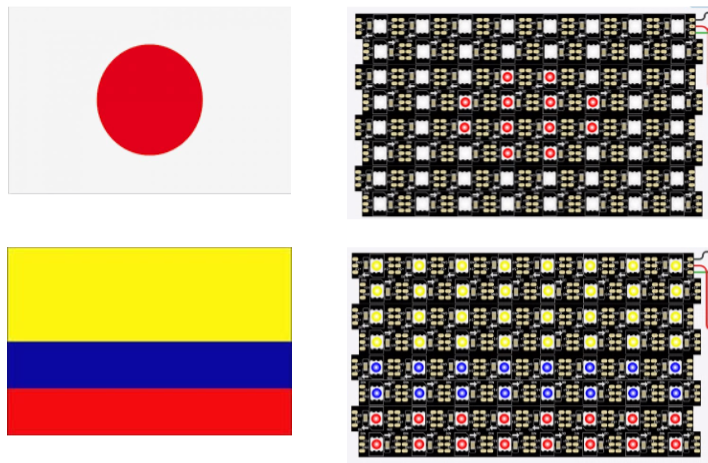
\includegraphics[width=10cm]{punto1banderas.png}
\centering
\caption{Ejemplo de representación.}
\label{fig:punto1}
\end{figure}

El programa recibirá la ubicación de la imagen de la bandera, la cual podrá tener cualquier tamaño, y después de hacer el debido procesamiento de esta, tendrá como salida un archivo de texto en el que se escribirá el código que debe ser utilizado en el controlador de la matriz que será copiado y pegado del archivo txt al programa en Tinkercad y que finalmente, al simular, se vea representada la imagen deseada por el usuario.

Para este cometido se tendrán que utilizar los conceptos vistos hasta el momento, como el manejo de archivos para lectura y escritura, la creación de clases y objetos, la noción de herencia y el montaje de circuitos haciendo uso del Arduino en el programa de modelado 3D Tinkercad.

Teniendo en cuenta que es permitido usar la clase QImage, la cual se encarga de manipular y proporcionar acceso a los pixeles de cualquier imagen, permitiendo de esta forma conocer la composición del color de cada pixel de la imagen suministrada por el usuario utilizando el modelo RGB, el principal objetivo en este ejercicio es encontrar la forma de reducir o aumentar el tamaño de cualquier imagen al deseado (16x16) que es el tamaño que se escogió implementar para la matriz de LEDs.

Por último, es importante que el segmento de código necesario para rellenar la matriz de LEDs con los colores correspondientes a la imagen, y que es proporcionado por el programa implementado en Qt, sea escrito de una forma en la que sea fácil de copiar en el programa que controla la matriz, para así evitar errores en la simulación y que no sea posible visualizar los colores en los LEDs.


\subsection{Clases implementadas}
\begin{enumerate}
\item Clase MatrizRGB: clase para mostrar las matrices que hacen parte de RGB
\item Clase newMatriz: Rellenar matriz redimensionada con nuevos valores


\end{enumerate}

\section{Tareas para la solución del problema} \label{tareas}
\begin{enumerate}
\item Entender el funcionamiento y las variedades de métodos de la clase QImage, la cual nos permitirá tener acceso a los pixeles de la imagen que queramos procesar, y de esta forma conocer la composición de color de estos.
\item Conocer el manejo de archivos haciendo uso de lenguaje C++, pues será nesesario para la salida del programa que se va a crear para solucionar el problema.
\item Idear una forma de minimizar o maximizar el tamaño de la imagen original dependiendo de sus dimensiones para que se convierta en una imagen de 16x16. Los colores de la nueva imagen serán creados a partir de las tres matrices que nos son dadas por el modelo RGB de la imagen original, tomando cada una de estas y minimizándolas o maximizándolas según lo requerido.
\item Se tendrá que realizar el montaje de una matriz de LEDs de 16x16 en la plataforma de simulaciones de Tinkercad haciendo uso de las tiras de Neopixeles.
\item Se debe crear un código en Tinkercad que controle la matriz de LEDs y que además sea fácil de cambiar por el usuario, pues él deberá tomar la información dada por el programa en C++ y pegarla en cierta parte del código para que de esta forma, la implementación en Tinkercad, muestre los colores deseados en la matriz de LEDs.


\end{enumerate}

\newpage
\section{Algoritmo diseñado} \label{algorimo}
\begin{figure}[h]
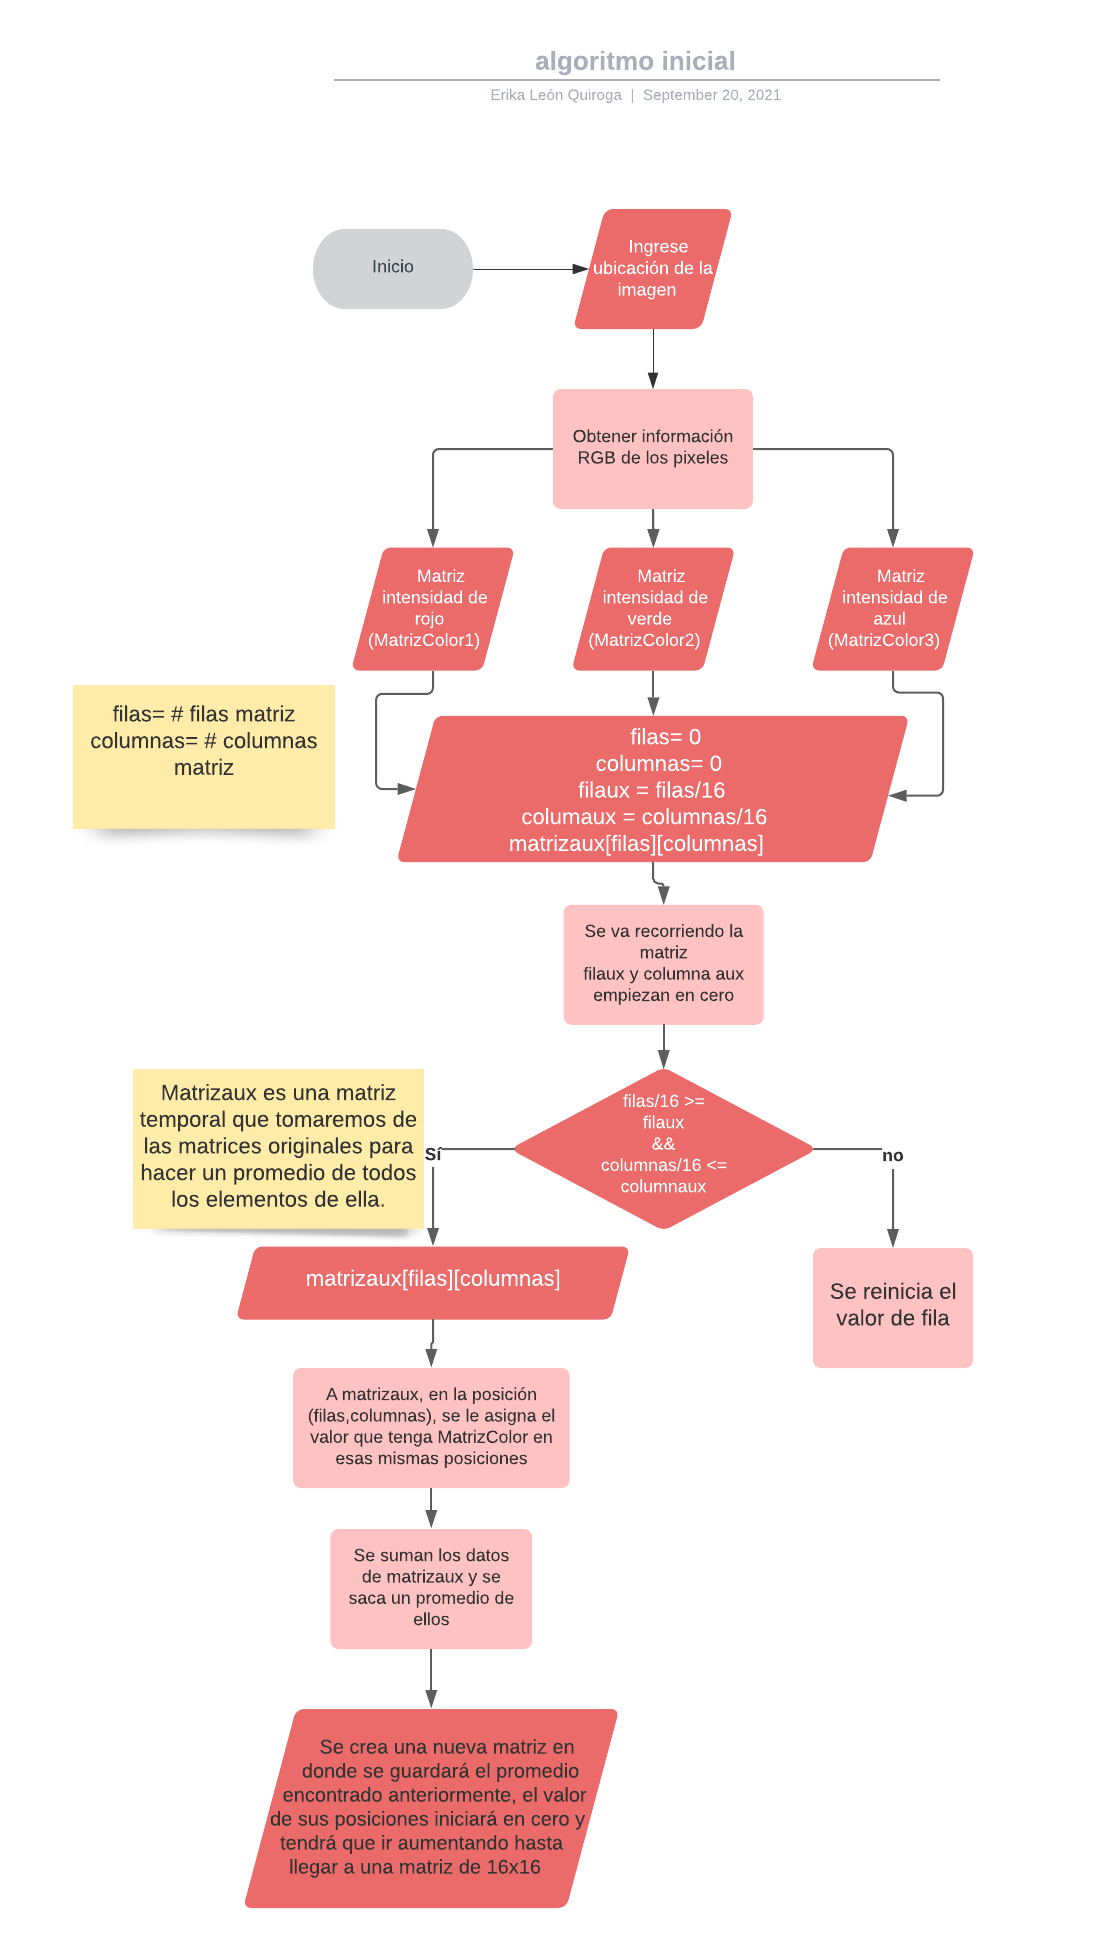
\includegraphics[width=15cm]{algoritmo.png}
\centering
\caption{Algoritmo inicial.}
\label{fig:algoritmo}
\end{figure}

\newpage
\section{Consideraciones finales} \label{consideracionesfinales}


\end{document}
